\documentclass[../sparc.tex]{subfiles}
\graphicspath{{\subfix{../images/}}}
\begin{document}

%%%%%%%%%%%%%%%%%%%%%%%%%%%%%%%%%%%%%%%%%%%%%%%%%%%%%%%%%%%%%%%%%%%%%%%%%%%%%%%%
\section{Подключение динамика}

Есть несколько вариантов динамиков, которые вы можете встретить.  Например, есть
обычные динамики, где мембрана колеблется под воздействием магнитного поля и тем
самым создаёт колебания воздуха, которые мы слышим как звук.  Также существуют
пьезодинамики, в которых звук генерируется за счёт обратного пьезоэлектрического
эффекта -- механической деформации пьезоэлектрика под действием электрического
поля.\footnote{См. статью ``Пьезоэлектрический эффект'' в Википедии для более
подробного описания эффекта.}

Подключение и обычных динамиков и пьезодинамиков похоже; для наших задач
подойдёт как пьезодинамик ``для Arduino'', так и обычный динамик-пищалка из
персонального компьютера (а вы знали, что у вас в компьютере к системной плате
подключен динамик?)

Схема подключения представлена на рис. \ref{fig:sound-fig-2}.

%% TODO: Перерисовать схему.  Убрать резистор.
\begin{figure}[h]
  \caption{Подключение динамика-''пищалки'' к Arduino Mega 2560.}
  \label{fig:sound-fig-2}
  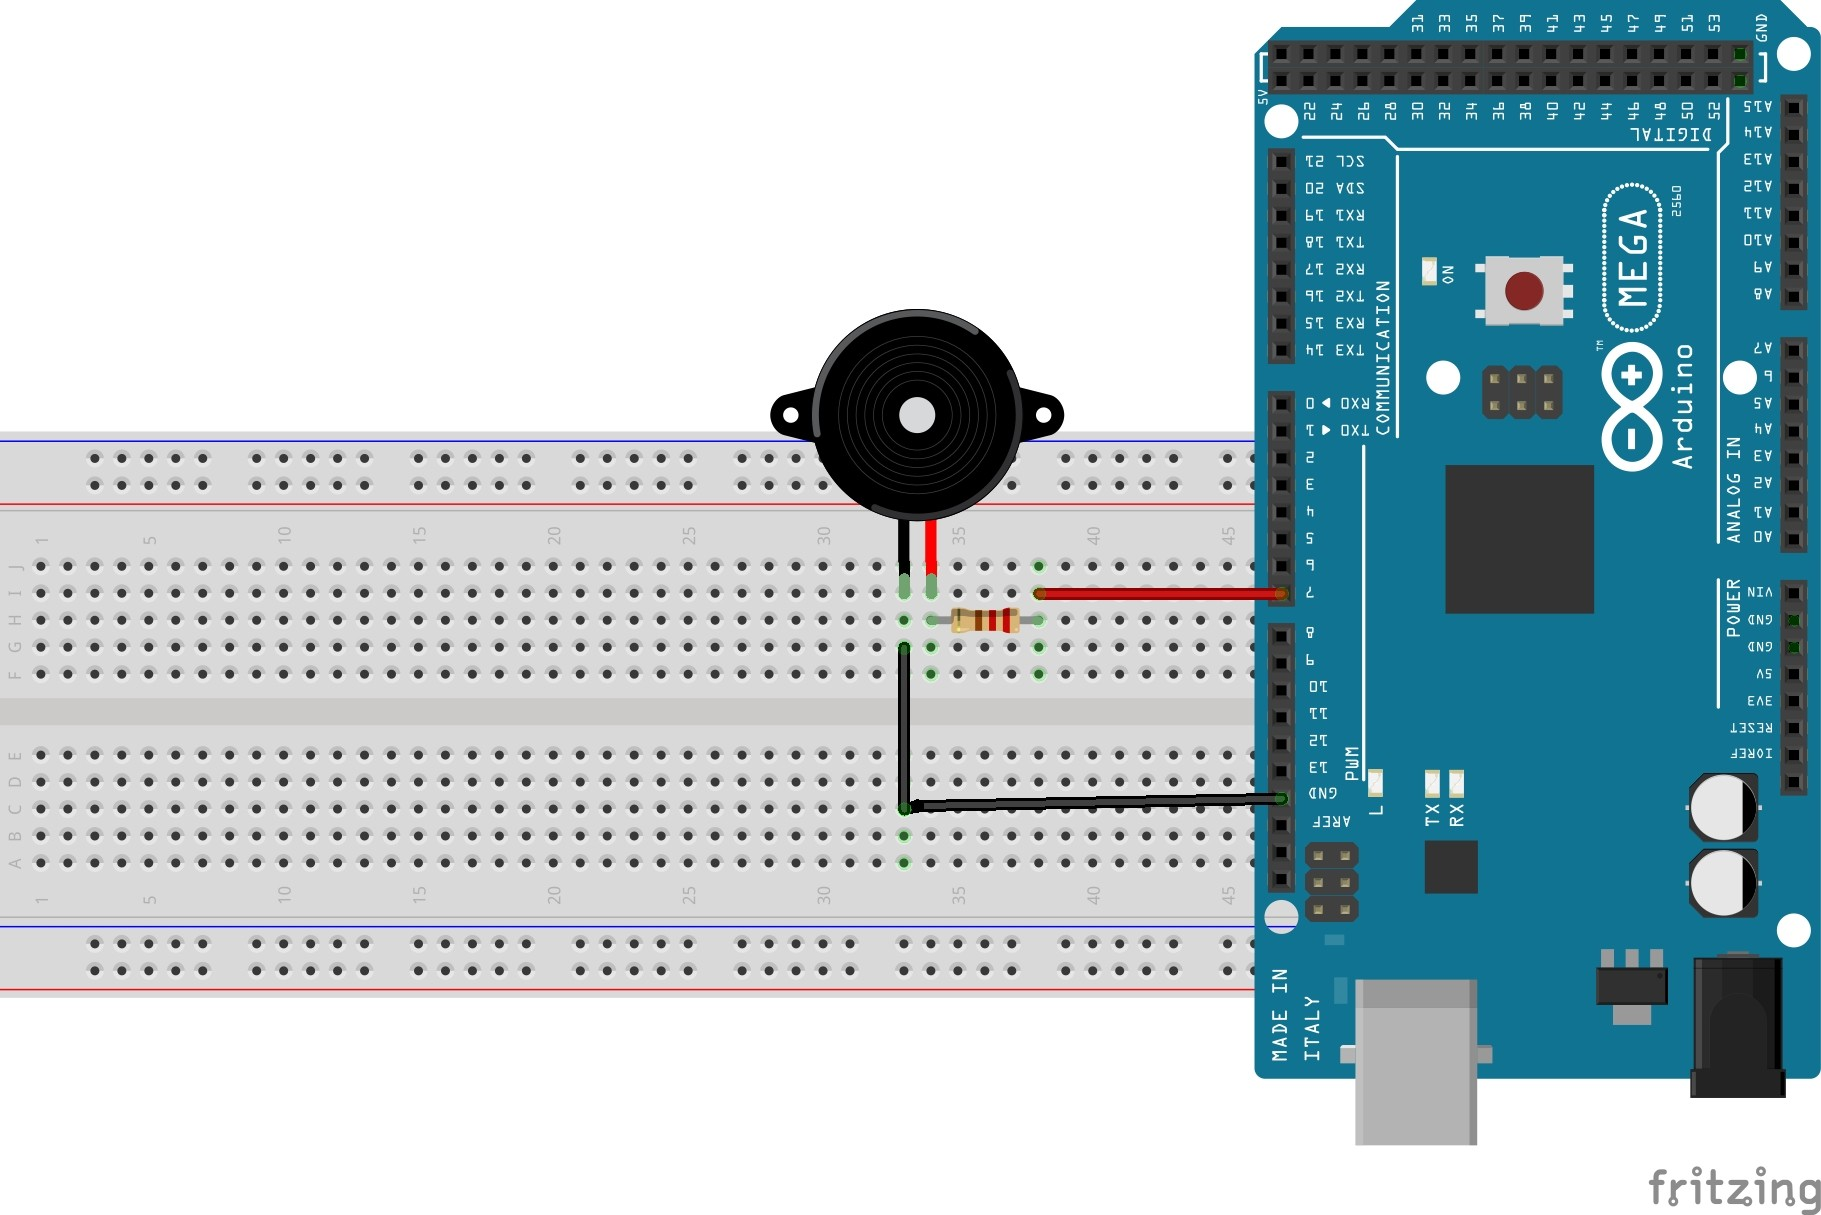
\includegraphics[width=10cm]{sound-fig-2}
  \centering
\end{figure}

Соберём указанную схему на макетной плате, и загрузим нашу программу генерации
звука в Arduino. Не забудьте добавить в тело функции \texttt{loop} вызов нашей
функции \texttt{play\_tone} и настроить цифровой порт, к которому подключен
динамик, на вывод.

Порт, к которому подключен динамик, лучше задать в виде константы
\texttt{SPEAKER\_PIN} в самом начале программы (до функции \texttt{setup}.)

\subsection{Задачи}
\begin{enumerate}
\item Сгенерируйте постоянный сигнал с частотой 261.63 Гц.
\item Сделайте так, чтобы сигнал менялся между 261.63 Гц и 349.23 Гц с частотой
  в 1 секунду.
\item Модифицируйте систему таким образом, чтобы частота сигнала зависела от
  положения ручки потенциометра.
\item Сделайте включение звукового сигнала по нажатию кнопки.
\end{enumerate}

Теперь мы можем генерировать звуковой сигнал с нужной нам частотой.  Однако,
если мы хотим сгенерировать что-нибудь интересное (например, мелодию), то нам
потребуется использовать определённые частоты.  В данном случае желательным
будет хотя бы начальное знание музыкальной теории, но такового нет -- не беда,
разберёмся по ходу дела.

\end{document}
